%---------------------------------------------------------------------
% Course 	: Introduction To web sciences
% Professor : Dr.Nelson
% Name   	: Babitha Bokka
% Assignment: 8
%---------------------------------------------------------------------
\documentclass[12pt]{article}
%--------------------------------------------------------------------
% packages required
%--------------------------------------------------------------------
\usepackage{graphicx}
\usepackage{listings}
\usepackage{hyperref}
\usepackage{caption}
\usepackage{color}
\usepackage{pdfpages}
\graphicspath{ {images/} }
%--------------------------------------------------------------------
% Start Margins
%--------------------------------------------------------------------
\addtolength{\oddsidemargin}{-.875in}
\addtolength{\evensidemargin}{-.875in}
\addtolength{\textwidth}{1.75in}
\addtolength{\topmargin}{-.885in}
\addtolength{\textheight}{1.95in}
%-------------------------------------------------------------------
% End Margins
%--------------------------------------------------------------------
\definecolor{codegreen}{rgb}{0,0.6,0}
\definecolor{codegray}{rgb}{0.5,0.5,0.5}
\definecolor{codepurple}{rgb}{0.58,0,0.82}
\definecolor{backcolour}{rgb}{0.95,0.95,0.92}
 
\lstdefinestyle{mystyle}{
    backgroundcolor=\color{backcolour},   
    commentstyle=\color{codegreen},
    keywordstyle=\color{magenta},
    numberstyle=\tiny\color{codegray},
    stringstyle=\color{codepurple},
    basicstyle=\footnotesize,
    breakatwhitespace=false,         
    breaklines=true,                 
    captionpos=b,                    
    keepspaces=true,                 
    numbers=left,                    
    numbersep=5pt,                  
    showspaces=false,                
    showstringspaces=false,
    showtabs=false,                  
    tabsize=2
}
 
\lstset{style=mystyle}

\begin{document}

%---------------------------------------------------------------------
%Making the title page
%---------------------------------------------------------------------
\begin{titlepage}
\title{INTRODUCTION TO WEB SCIENCES:\\*Assignment 8}
\author{Babitha Bokka}
\date{15 November 2014}
\maketitle
\end{titlepage}

%---------------------------------------------------------------------
%Table of contents
%---------------------------------------------------------------------
\tableofcontents
\newpage
%------------------------------------------------------------------
%Question 1
%------------------------------------------------------------------
\section{Question 1:}
What 5 movies have the highest average ratings? Show the movies
and their ratings sorted by their average ratings.
%-----------------------Approach----------------------------------
\subsection{Approach}
\begin{enumerate}
    \item To solve this question the straight forward approach is to read u.data file get movie id, corresponding movie ratings and read u.item file to get movie id and corresponding movie name.
    \item Extract the movie id and ratings. For each movie id build a dictionary that has all the ratings.
    \item Now, for each movie id calculate the average using sum() and len() functions.
    \item For each movie id get the movie name and append it to the dictionary which has average.
    \item Now, sort the dictionary and print the top 5 movies with highest average ratings.
    \item Program averageMovies.py produces the top 5 movies with highest average ratings. The output is based on a condition which can be changed accordingly.
    \item Figure~\ref{fig:averageMovies} shows the results of the program. 
\end{enumerate}
   
\newpage
%-----------------------Source Code-------------------------------
\subsection{Source Code}
\subsubsection{averageMovies.py}
\lstinputlisting[breaklines=True,language=Python]{../Q1/averageMovies.py}
\newpage

\subsection{Input Files}
\subsubsection{u.data}
\lstinputlisting[breaklines=True]{../u.dataForDoc}
\subsubsection{u.item}
\lstinputlisting[breaklines=True]{../u.itemForDoc}

\newpage
%-----------------------Output Section---------------------------
\subsection{Output Files}
\subsubsection{averageMovies.png}
\begin{figure}[ht]
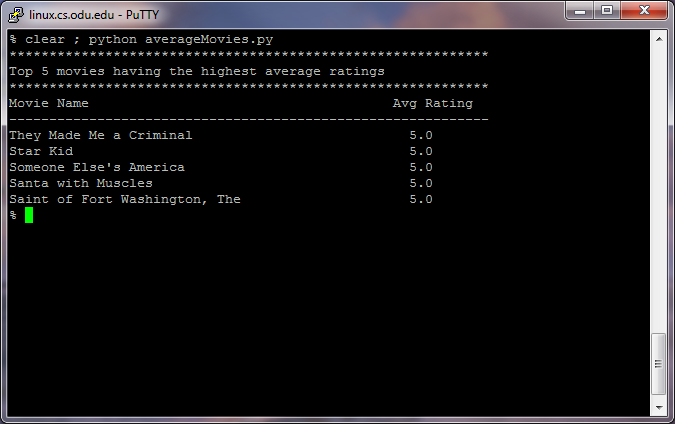
\includegraphics[scale=1.0]{../Q1/averageMovies}
\centering
\caption{Top 5 movies with highest average ratings.}
\label{fig:averageMovies}
\end{figure}
\newpage
\subsubsection{averageMoviesMore.txt}
Movies with highest average ratings. The above output shows only top 5 but the below output shows all the movies with the same average ratings.
\lstinputlisting[breaklines=True]{../Q1/averageMoviesMore.txt}
\newpage
%------------------------------------------------------------------
%Question 2
%------------------------------------------------------------------
\section{Question 2:}
What 5 movies received the most ratings? Show the movies and
the number of ratings sorted by number of ratings.
%-----------------------Approach----------------------------------
\subsection{Approach}
\begin{enumerate}
    \item The approach is same as question 1. 
    \item The only difference is we count the number of ratings for each movie and display the corresponding movie name and number of ratings for each movie.
    \item The output displays only top 5 movies and their number of ratings. 
    \item Figure~\ref{fig:mostRatingMovies} is the output for the program.
\end{enumerate}


\newpage
%-----------------------Source Code-------------------------------
\subsection{Source Code}
\subsubsection{mostRatingMovies.py}
\lstinputlisting[breaklines=True,language=Python]{../Q2/mostRatingMovies.py}
\newpage

%-----------------------Input Section---------------------------
\subsection{Input Files}
\subsubsection{u.data}
\lstinputlisting[breaklines=True]{../u.dataForDoc}
\subsubsection{u.item}
\lstinputlisting[breaklines=True]{../u.itemForDoc}
\newpage

%-----------------------Output Section---------------------------
\subsection{Output Files}
\subsubsection{mostRatingMovies.png}
\begin{figure}[ht]
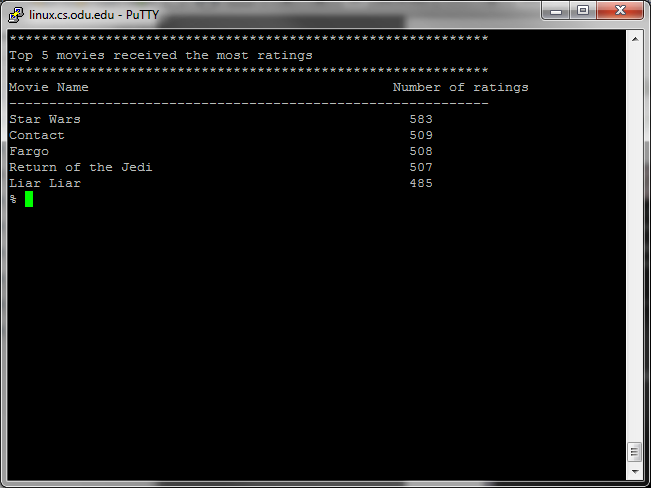
\includegraphics[scale=1.0]{../Q2/mostRatingMovies}
\centering
\caption{Top 5 movies received the most ratings.}
\label{fig:mostRatingMovies}
\end{figure}
\newpage

%------------------------------------------------------------------
%Question 
%------------------------------------------------------------------
\section{Question 3:}
What 5 movies were rated the highest on average by women? Show
the movies and their ratings sorted by ratings.

%-----------------------Approach----------------------------------
\subsection{Approach}
\begin{enumerate}
    \item To solve this question the straight forward approach is to read u.user file get the user id, gender. Read u.data file get movie id, corresponding movie ratings. Read u.item file to get movie id and corresponding movie name.
	\item From u.user file extract the user id and gender store them in a dictionary.     
    \item Now, Extract the movie id and ratings. For each user id build a dictionary that has all the ratings for the respective gender.
    \item Now, for each movie id calculate the average a using sum() and len() functions.
    \item For each movie id get the movie name and append it to the dictionary which has average.
    \item Now, sort the dictionary and print the top 5 movies rated the highest on average by women.
    \item Program averageGender.py is designed in  such a way that it can get the highest averages by men and women just by changing the arguments to F or M while executing the program.
    \item Figure~\ref{fig:averageGenderF} is the output showing top 5 movies rated the highest on average by women. The results of the program are limited to  top 5 it can be modified to get more average ratings. 
\end{enumerate}


\newpage
%-----------------------Source Code-------------------------------
\subsection{Source Code}
\subsubsection{averageMovies.py}
\lstinputlisting[breaklines=True,language=Python]{../Q3/averageGender.py}
\newpage

%-----------------------Input Section---------------------------
\subsection{Input Files}
\subsubsection{u.data}
\lstinputlisting[breaklines=True]{../u.dataForDoc}
\subsubsection{u.item}
\lstinputlisting[breaklines=True]{../u.itemForDoc}
\subsubsection{u.user}
\lstinputlisting[breaklines=True]{../u.userForDoc}
\newpage

%-----------------------Output Section---------------------------
\subsection{Output Files}
\subsubsection{averageGenderF.png}
\begin{figure}[ht]
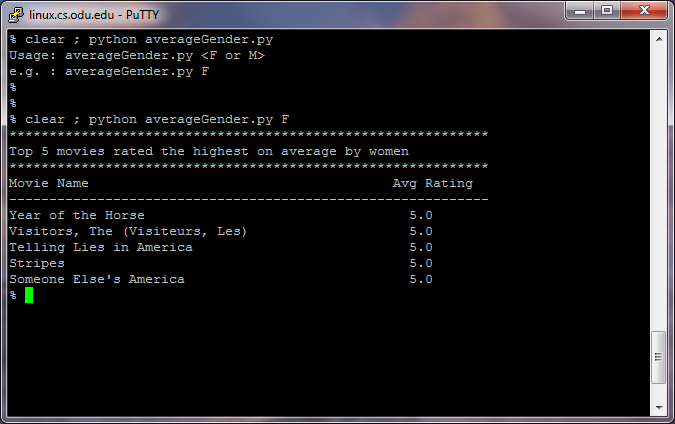
\includegraphics[scale=1.0]{../Q3/averageGenderF}
\centering
\caption{Top 5 movies rated the highest on average by women.}
\label{fig:averageGenderF}
\end{figure}
\newpage
\subsubsection{averageGenderFull.txt}
Showing all the movies with same average ratings.
\lstinputlisting[breaklines=True]{../Q3/averageGenderFull.txt}
\newpage
%------------------------------------------------------------------
%Question 4
%------------------------------------------------------------------
\section{Question 4:}
What 5 movies were rated the highest on average by men? Show
the movies and their ratings sorted by ratings.
%-----------------------Approach----------------------------------
\subsection{Approach}
\begin{enumerate}
    \item The approach is same as question 3. 
    \item The only difference is changing the command line argument which can be seen in the output produced. 
    \item The output displays only top 5 movies rated the highest on average by men.
    \item Figure~\ref{fig:averageGenderM} is the output for the program.
\end{enumerate}

\newpage
%-----------------------Source Code-------------------------------
\subsection{Source Code}
\subsubsection{averageMovies.py}
\lstinputlisting[breaklines=True,language=Python]{../Q3/averageGender.py}
\newpage

%-----------------------Input Section---------------------------
\subsection{Input Files}
\subsubsection{u.data}
\lstinputlisting[breaklines=True]{../u.dataForDoc}
\subsubsection{u.item}
\lstinputlisting[breaklines=True]{../u.itemForDoc}
\subsubsection{u.user}
\lstinputlisting[breaklines=True]{../u.userForDoc}
\newpage

%-----------------------Output Section---------------------------
\subsection{Output Files}
\subsubsection{averageGenderM.png}
\begin{figure}[ht]
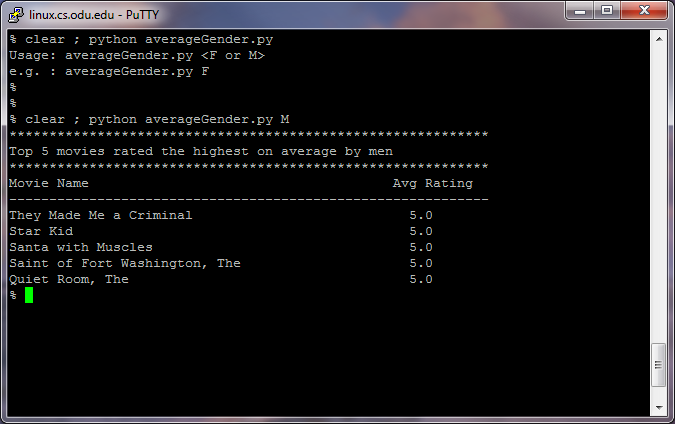
\includegraphics[scale=1.0]{../Q4/averageGenderM}
\centering
\caption{Top 5 movies rated the highest on average by men.}
\label{fig:averageGenderM}
\end{figure}
\newpage
\subsubsection{averageGenderFull.txt}
Showing all the movies with same average ratings.
\lstinputlisting[breaklines=True]{../Q4/averageGenderFull.txt}
\newpage
%------------------------------------------------------------------
%Question 5
%------------------------------------------------------------------

\section{Question 5:}
What movie received ratings most like Top Gun? Which movie
received ratings that were least like Top Gun (negative correlation)?
%-----------------------Approach----------------------------------
\subsection{Approach}

\subsection{Approach}
\begin{enumerate}
\item To solve question 5 we need recommendation.py.
\item To get the desired output I modified calculateSimilarItems()and loadMovieLens() functions.
\item The file ratingsLikeTopGun.txt shows the output for movies having ratings most like Top Gun.
\item The file ratingsLeastTopGun.txt shows the output for movies having ratings least like Top Gun.
\item To see more results run ratingsTopGun.py.

 
     
\end{enumerate}

\newpage
%-----------------------Source Code-------------------------------
\subsection{Source Code}
\subsubsection{recommendations.py}
\lstinputlisting[breaklines=True,language=Python]{../Q5/reForDoc.py}
\newpage
\subsubsection{ratingsTopGun.py}
\lstinputlisting[breaklines=True,language=Python]{../Q5/ratingsTopGun.py}
\newpage

%-----------------------Input Section---------------------------
\subsection{Input Files}
\subsubsection{u.data}
\lstinputlisting[breaklines=True]{../u.dataForDoc}
\subsubsection{u.item}
\lstinputlisting[breaklines=True]{../u.itemForDoc}
\newpage

%-----------------------Output Section---------------------------
\subsection{Output Files}
\subsubsection{ratingsLikeTopGun.txt}
\lstinputlisting[breaklines=True]{../Q5/ratingsLikeTopGun.txt}
\newpage
\subsubsection{ratingsLeastTopGun.txt}
\lstinputlisting[breaklines=True]{../Q5/ratingsLeastTopGun.txt}
\newpage
%------------------------------------------------------------------
%Question 6
%------------------------------------------------------------------

\section{Question 6:}
Which 5 raters rated the most films? Show the raters' IDs and
the number of films each rated.
%-----------------------Approach----------------------------------
\subsection{Approach}

\begin{enumerate}
    \item The approach for this question is modify question 1 to read U.data file, get user id and for the corresponding user id store all the ratings . 
    \item Now, we count the number of ratings for each user by using the len() function.
    \item The output displays only top 5 users and their number of ratings. 
    \item Figure~\ref{fig:ratersMostRatedMovies} is the output for the program.
\end{enumerate}
\newpage
%-----------------------Source Code-------------------------------
\subsection{Source Code}
\subsubsection{ratersMostRatedMovies.py}
\lstinputlisting[breaklines=True,language=Python]{../Q6/ratersMostRatedMovies.py}
\newpage

\subsection{Input Files}
\subsubsection{u.data}
\lstinputlisting[breaklines=True]{../u.dataForDoc}

%-----------------------Output Section---------------------------
\subsection{Output Files}
\subsubsection{ratersMostRatedMovies.png}
\begin{figure}[ht]
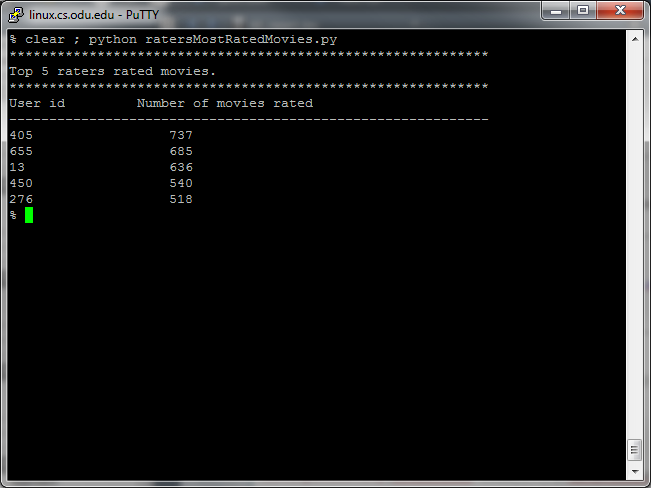
\includegraphics[scale=1.0]{../Q6/ratersMostRatedMovies}
\centering
\caption{Top 5 raters rated movies.}
\label{fig:ratersMostRatedMovies}
\end{figure}
\newpage
%------------------------------------------------------------------
%Question 7
%------------------------------------------------------------------
\section{Question 7:}
Which 5 raters most agreed with each other? Show the raters'
IDs and Pearson's r, sorted by r.
%-----------------------Approach----------------------------------
\subsection{Approach}
I couldn't complete this question.
\subsection{Description of}


%-----------------------Source Code-------------------------------
\subsection{Source Code}

%-----------------------Input Section---------------------------


%-----------------------Output Section---------------------------
\subsection{Output Files}

\newpage
%------------------------------------------------------------------
%Question 8
%------------------------------------------------------------------
\section{Question 8:}
 Which 5 raters most disagreed with each other (negative
correlation)? Show the raters' IDs and Pearson's r, sorted by r.
%-----------------------Approach----------------------------------
\subsection{Approach}
I couldn't complete this question.
\subsection{Description of}


%-----------------------Source Code-------------------------------
\subsection{Source Code}

%-----------------------Input Section---------------------------


%-----------------------Output Section---------------------------
\subsection{Output Files}

\newpage
%------------------------------------------------------------------
%Question 9
%------------------------------------------------------------------
\section{Question 9:}
What movie was rated highest on average by men over 40? By men
under 40?
%-----------------------Approach----------------------------------
\subsection{Approach}
\begin{enumerate}
\item To solve this question, the straight forward approach is to read u.user file, get the user id, gender, age of each user. Read u.data file, get movie id, corresponding movie ratings. Read u.item file to get movie id and corresponding movie name.
	\item Program averageOverUnderGender.py is designed in  such a way that it can get the highest averages by men and women over and under 40 just by changing the arguments to F or M  and ``over'' or ``under'' while executing the program.	
	\item From u.user file extract the user id, gender, age,  based on arguments given from command line either men over 40 or men under 40 or women over 40 or women under 40 is stored into dictionary.     
    \item Now, Extract the movie id and ratings. For each user id build a dictionary that has all the ratings for the respective gender with over or under condition.
    \item Now, for each movie id calculate the average a using sum() and len() functions.
    \item For each movie id get the movie name and append it to the dictionary which has average.
    \item Now, sort the dictionary and get the movies which are rated highest on average by men or women over 40 or under 40.
    \item  Figure~\ref{fig:averageOverM} is the output showing how to execute the program and displays the top 5 movies which are rated highest on average by men ``over'' 40.
    \item  Figure~\ref{fig:averageUnderM} is the output showing how to execute the program and displays the top 5 movies which are rated highest on average by men ``under'' 40.
    \item  The file averageOverM.txt and averageUnderM.txt displays movies which have the same average ratings.     
     
\end{enumerate}

\newpage
%-----------------------Source Code-------------------------------
\subsection{Source Code}
\subsubsection{averageOverUnderGender.py}
\lstinputlisting[breaklines=True,language=Python]{../Q9/averageOverUnderGender.py}
\newpage

%-----------------------Input Section---------------------------
\subsection{Input Files}
\subsubsection{u.data}
\lstinputlisting[breaklines=True]{../u.dataForDoc}
\subsubsection{u.item}
\lstinputlisting[breaklines=True]{../u.itemForDoc}
\subsubsection{u.user}
\lstinputlisting[breaklines=True]{../u.userForDoc}
\newpage

%-----------------------Output Section---------------------------
\subsection{Output Files}
\subsubsection{averageOverM.png}
\begin{figure}[ht]
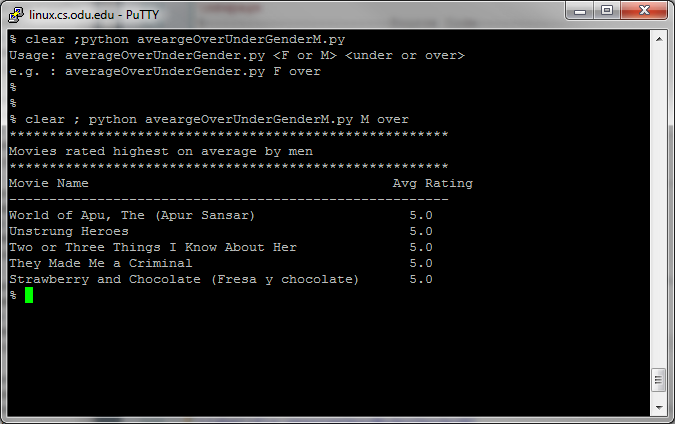
\includegraphics[scale=1.0]{../Q9/averageOverM}
\centering
\caption{Movies rated highest on average by men over 40.}
\label{fig:averageOverM}
\end{figure}
\newpage
\subsubsection{averageUnderM.png}
\begin{figure}[ht]
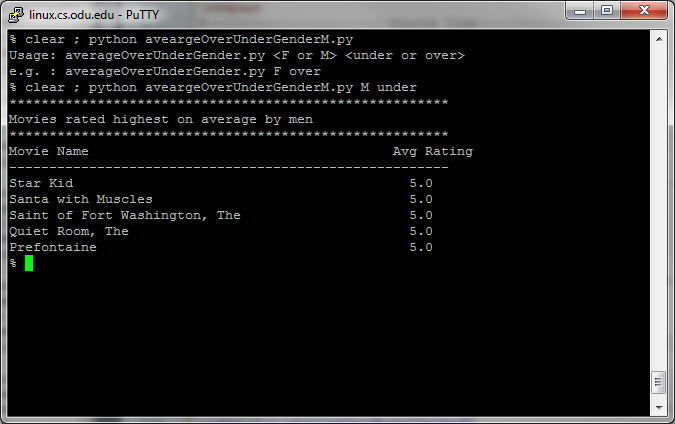
\includegraphics[scale=1.0]{../Q9/averageUnderM}
\centering
\caption{Movies rated highest on average by men under 40.}
\label{fig:averageUnderM}
\end{figure}
\newpage
\subsubsection{averageOverM.txt}
\lstinputlisting[breaklines=True]{../Q9/averageOverM.txt}
\newpage
\subsubsection{averageUnderM.txt}
\lstinputlisting[breaklines=True]{../Q9/averageUnderM.txt}
\newpage
%------------------------------------------------------------------
%Question 10
%------------------------------------------------------------------
\section{Question 10:}
What movie was rated highest on average by women over 40? By
women under 40?
%-----------------------Approach----------------------------------
\subsection{Approach}

\begin{enumerate}
    \item The approach is same as question 9.
     
    \item To get the corresponding output for this question it will still use averageOverUnderGender.py but the only difference is  changing the arguments.  
      
     \item  Figure~\ref{fig:averageOverF} is the output showing how to execute the program and displays the top 5 movies which are rated highest on average by men ``over'' 40.
    \item  Figure~\ref{fig:averageUnderF} is the output showing how to execute the program and displays the top 5 movies which are rated highest on average by men ``under'' 40.
       \item  The file averageOverF.txt and averageUnderF.txt displays movies which have the same average ratings.
    
\end{enumerate}

\newpage
%-----------------------Source Code-------------------------------
\subsection{Source Code}
\subsubsection{averageOverUnderGender.py}
\lstinputlisting[breaklines=True,language=Python]{../Q10/averageOverUnderGender.py}
\newpage
%-----------------------Input Section---------------------------
\subsection{Input Files}
\subsubsection{u.data}
\lstinputlisting[breaklines=True]{../u.dataForDoc}
\subsubsection{u.item}
\lstinputlisting[breaklines=True]{../u.itemForDoc}
\subsubsection{u.user}
\lstinputlisting[breaklines=True]{../u.userForDoc}
\newpage
%-----------------------Output Section---------------------------
\subsection{Output Files}
%----------------------over---------------------------------------
\subsubsection{averageOverF.png}
\begin{figure}[ht]
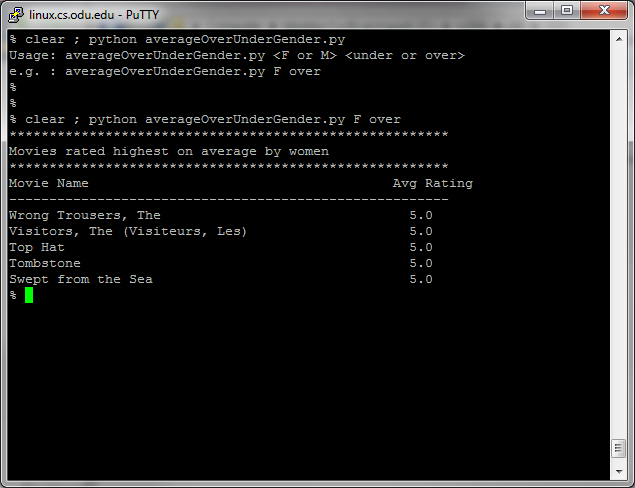
\includegraphics[scale=1.0]{../Q10/averageOverF}
\centering
\caption{Movies rated highest on average by women over 40.}
\label{fig:averageOverF}
\end{figure}
\newpage
%--------------------- under--------------------------------------
\subsubsection{averageUnderF.png}
\begin{figure}[ht]
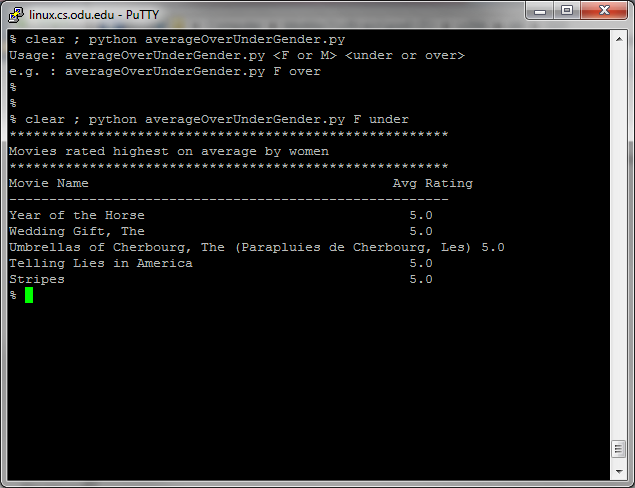
\includegraphics[scale=1.0]{../Q10/averageUnderF}
\centering
\caption{Movies rated highest on average by women under 40.}
\label{fig:averageUnderF}
\end{figure}
\newpage
\subsubsection{averageOverF.txt}
\lstinputlisting[breaklines=True]{../Q10/averageOverF.txt}
\newpage
\subsubsection{averageUnderF.txt}
\lstinputlisting[breaklines=True]{../Q10/averageUnderF.txt}
\newpage
%-----------------------End Question 10---------------------------
%------------------------------------------------------------------
%Bibilography
%------------------------------------------------------------------
\bibliographystyle{plain}
\bibliography{A8_report}
\cite{*}

\end{document}